\newpage
\section{Análise em regime subsônico}

Os dois aerofólios foram exportados para o Xfoil e analisados em regime
viscoso subsônico na condição de decolagem. O Reynolds, calculado com a
corda da seção de referência na velocidade de decolagem, é
$Re = 4{,}23 \times 10^{7}$; o número de Mach foi desprezado, como permite o
roteiro. Os painéis foram redistribuídos com o comando \texttt{PPAR} após a
carga de cada geometria, como recomendado, e a análise viscosa usou
$N_{\mathrm{crit}} = 9$ com varredura de $\alpha$ de $-6^\circ$ a
$+28^\circ$ em passos de $0{,}5^\circ$ --- a varredura precisa ir longe o
suficiente para capturar o estol, que nesses Reynolds ocorre acima de
$20^\circ$. As Figuras~\ref{fig:cl_alpha} a~\ref{fig:cm_alpha} sobrepõem as
curvas dos dois perfis.

\begin{figure}[H]
    \centering
    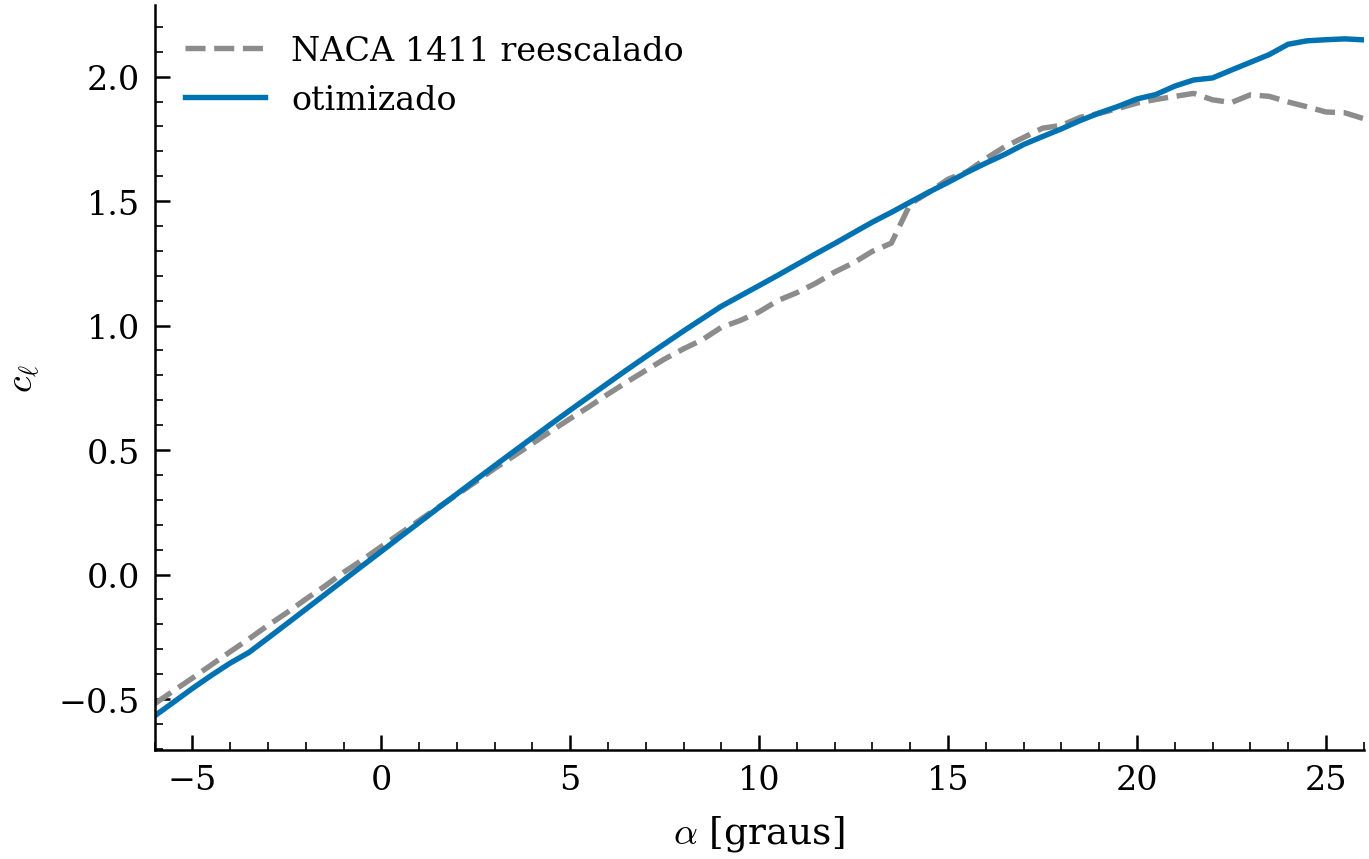
\includegraphics[width=0.8\textwidth]{images/07_subsonico/cl_alpha.png}
    \caption{$c_\ell \times \alpha$ dos perfis inicial (NACA~1411
    reescalado) e otimizado no regime subsônico
    ($Re = 4{,}23\times10^{7}$).}\label{fig:cl_alpha}
\end{figure}

\begin{figure}[H]
    \centering
    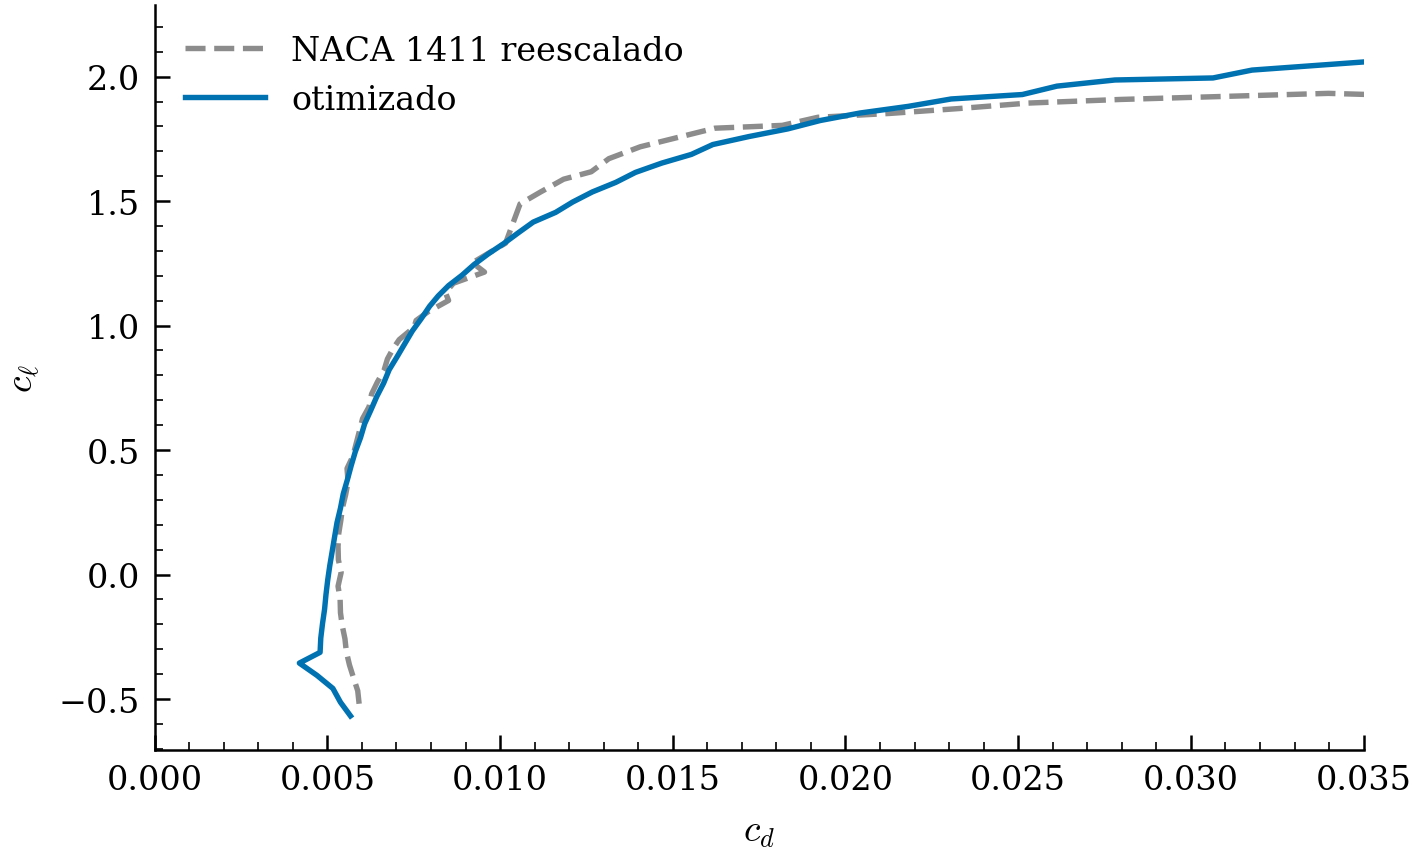
\includegraphics[width=0.8\textwidth]{images/07_subsonico/cl_cd.png}
    \caption{Polar $c_\ell \times c_d$ dos perfis inicial e otimizado no
    regime subsônico.}\label{fig:cl_cd}
\end{figure}

\begin{figure}[H]
    \centering
    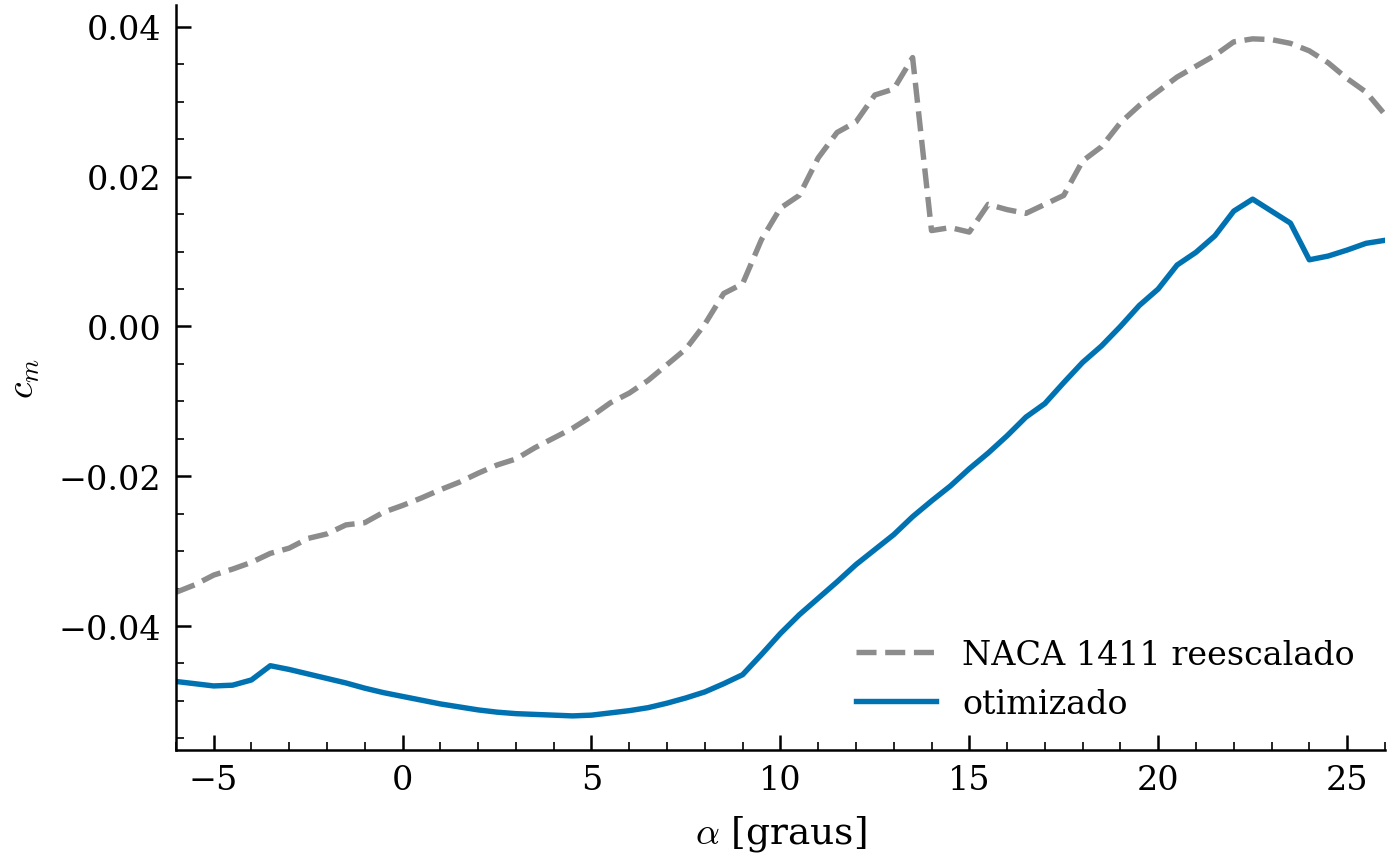
\includegraphics[width=0.8\textwidth]{images/07_subsonico/cm_alpha.png}
    \caption{$c_m \times \alpha$ dos perfis inicial e otimizado no regime
    subsônico.}\label{fig:cm_alpha}
\end{figure}

O quadro comparativo é favorável ao otimizado em quase tudo. A inclinação
da curva de sustentação sobe de $0{,}105$ para $0{,}115$/grau; o
$c_{\ell,\max}$ sobe de $1{,}93$ para $2{,}15$, com estol adiado de
$21{,}5^\circ$ para $25{,}5^\circ$; e o arrasto mínimo cai de $0{,}0053$
para $0{,}0042$. Vale registrar que o Xfoil superestima $c_{\ell,\max}$
nesses Reynolds: aferindo o método contra dados experimentais de cinco
perfis NACA (Abbott \& von Doenhoff), medimos um viés sistemático de
$+0{,}24$; descontado, o otimizado entrega $c_{\ell,\max} \approx 1{,}91$
--- ainda acima do $1{,}80$ assumido para \texttt{clmax\_w} no
dimensionamento da aeronave, confirmando que a restrição substituta da
Seção~4 cumpriu seu papel.

A desvantagem única, e relevante, é o momento picador: o $c_m$ médio na
faixa de voo mais que dobra, de $-0{,}022$ para $-0{,}050$ (e $-0{,}097$ na
condição transônica). É o preço direto do carregamento traseiro da
Seção~5, e será pago em arrasto de trimagem e em torção da asa --- um
custo a acompanhar nos próximos laboratórios, quando empenagem e torção
forem dimensionadas.

% ----- Atividade 9 -----
\subsection*{Adaptação da otimização para o regime subsônico}

A adaptação para o subsônico não foi um ajuste posterior: ela já está
embutida na formulação da Seção~4, na forma da restrição substituta
$t_{01}/\sqrt{(t/c)_{\max}} \ge 0{,}0938$. Para verificar se ela é
necessária e qual o seu custo, o mesmo problema foi resolvido em três
formulações, e a Tabela~\ref{tab:variantes} resume o resultado.

\begin{table}[H]
\centering
\caption{Efeito da formulação sobre o desempenho nos dois
regimes.}\label{tab:variantes}
\renewcommand{\arraystretch}{1.25}
\begin{tabular}{lcccc}
\toprule
Formulação & $c_d$ transônico & $c_{\ell,\max}$ (Xfoil) & $\alpha_{\mathrm{estol}}$ & $c_m$ médio \\
\midrule
Batentes do roteiro (adotada) & $0{,}01164$ & $2{,}15$ & $25{,}5^\circ$ & $-0{,}050$ \\
Sem restrição de $c_{\ell,\max}$ & $0{,}01066$ & $0{,}99$ & $8{,}6^\circ$ & $-0{,}032$ \\
Cusp liberado ($A_{l4} \le 0{,}30$) & $0{,}00822$ & $2{,}21$ & $23{,}5^\circ$ & $-0{,}091$ \\
\bottomrule
\end{tabular}
\end{table}

Duas conclusões. Primeiro, \textbf{a restrição substituta é indispensável}:
sem ela, o otimizador afia o nariz em busca dos últimos $8\%$ de arrasto
transônico e o perfil resultante estola a $8{,}6^\circ$ com
$c_{\ell,\max} = 0{,}99$ --- inviável para a decolagem, que exige
$c_{\ell,\max} \ge 1{,}80$ na seção. O custo dela é de $+9\%$ no arrasto
transônico, um seguro barato. Segundo, \textbf{o batente do roteiro em}
$A_{l4}$ \textbf{deixa desempenho na mesa deliberadamente}: liberando o
côncavo traseiro ($A_{l4} \le 0{,}30$), o otimizador constrói um
\emph{cusp} supercrítico pleno e o arrasto transônico cai mais $29\%$, com
$c_{\ell,\max}$ até maior --- mas o $c_m$ quase dobra de novo, para
$-0{,}091$ no subsônico. O batente é, na prática, uma restrição implícita
de momento picador. A decisão entre as duas formulações não pertence ao
perfil isolado: ela depende do custo de trimagem e de torção que a
aeronave completa pode pagar, e por isso mantivemos a formulação do
roteiro como resultado principal, deixando a variante com cusp documentada
como potencial de ganho para a próxima iteração do projeto.

\begin{figure}[H]
    \centering
    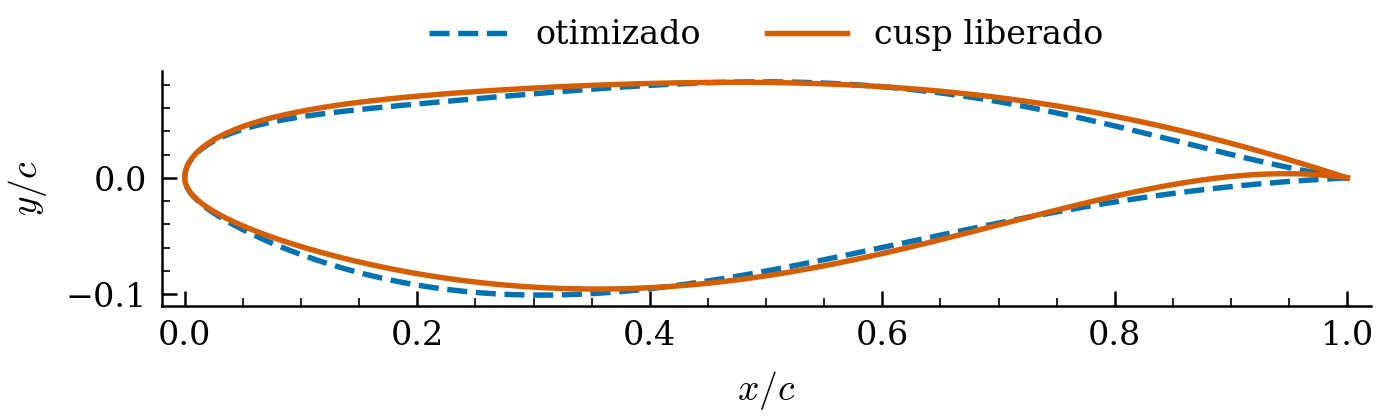
\includegraphics[width=0.8\textwidth]{images/05_transonico/geometria_item9.png}
    \caption{Geometria da variante com cusp liberado sobreposta à
    formulação adotada: o côncavo no intradorso traseiro é o
    \emph{cusp} supercrítico responsável pelos $-29\%$ de arrasto
    transônico --- e pelo dobro do momento picador.}\label{fig:geom_item9}
\end{figure}
